\section{Gezielte ergonomische Verbesserungen} \label{sec:analyse-ergo}

Die Kriterien von Bastien und Scapin haben sehr gezielte Lücken in der Benutzeroberfläche aufgedeckt.
Die Benutzertests zeigten verwirrendes Verhalten, das auf einen Mangel an intuitiver Usability hindeutet.
Dieser Teil konzentriert sich daher auf die Behebung von Mängeln im Zusammenhang mit der Fehlerbehandlung, die Anpassung der Benutzeroberfläche und die Einführung von UI-Konzepten, die eine einfache Entdeckung einer neuen Benutzeroberfläche ermöglichen.

\subsection{Intuitive Verwaltung und Design von Fehlern}

Es ist wichtig zu verstehen, dass \ac{UX} und \ac{UI} Hand in Hand gehen; man kann das eine nicht ohne das andere haben.
Wie Rahul Varshney so treffend zitiert hat: ``UX ohne UI ist wie der Rahmen einer Skulptur ohne Pappmaché darauf. Ein großartiges Produkterlebnis beginnt mit UX, gefolgt von UI. Beide sind für den Erfolg des Produkts unerlässlich.''.
Daher scheint es sinnvoll zu sein, dem Nutzer die freundlichste aller möglichen UIs anzubieten.
Aus Zeitgründen sollte man sich auf die Teile der Anwendung konzentrieren, die am meisten davon profitieren.
Dies gilt insbesondere für Seiten, auf denen sich der Nutzer verletzlich und gestresst fühlt. Ein gutes Beispiel sind Fehlerseiten.
Dies lässt sich damit begründen, dass Nutzer eine positive emotionale Reaktion auf visuelles Design haben, was sie toleranter gegenüber kleineren Problemen mit der Benutzerfreundlichkeit Ihrer Website macht \cite{aestheticEffect}.
Daher neigen Menschen dazu zu glauben, dass Dinge, die besser aussehen, auch besser funktionieren - auch wenn sie nicht wirklich effektiver oder effizienter sind.
Dieses Phänomen heißt \textit{Der Ästhetik-Nutzungs-Effekt}.

\subsubsection{Darstellung des Fehlers}

Ein Beispiel für eine in der Webwelt recht verbreitete Fehlerrückmeldung ist eine 404-Seite, die anzeigt, dass die vom Benutzer angeforderte Ressource nicht oder nicht mehr existiert.
Die Anwendung von Dryad hat eine solche dynamische Seite, die sich an die Art des Fehlers anpasst, enthält aber tiefe Mängel in Bezug auf \ac{UX} und \ac{UI}.

\begin{figure}[H]
  \centering
  
\includegraphics[width=\textwidth]{app_404_broken_error}
  \caption{Screenshot der Seite 404 der Schnittstelle}
  \label{fig:app_404_broken_error}
\end{figure}

Das Design ist völlig kaputt und es gibt keine Aktionen für den Benutzer, was zu einer schlechten Erfahrung führt.
Auch gibt es hier keine UI-Elemente, die die Ästhetik der Seite unterstützen sollen.
Um diese Art von Fehlerseite interessanter zu gestalten, wäre es sinnvoll, eine kleine animierte Illustration und eine Fallback-Aktion einzufügen, die dem Nutzer die Orientierung erleichtert.
Auch die Beschreibung des Fehlers könnte sympathischer gestaltet werden, indem man mit der Sensibilität des Nutzers spielt.
So könnte man sich für die Beschreibung einer 404-Seite vorstellen, "Die von Ihnen angeforderte Seite kann nicht gefunden werden" durch "Die von Ihnen gesuchte Seite kann umbenannt, gelöscht oder nie auf der Erde existieren" zu ersetzen.

Für die Illustrationen ist es sinnvoll, die bereits von Dryad erstellten Grafiken und Farben beizubehalten.
Die folgenden Illustrationen wurden mit dem Figma-Tool erstellt und werden jeweils von links nach rechts für eine nicht existierende Seite, den Zugriff auf eine Seite, die aufgrund fehlender Rechte verboten ist, und die Seite, die anzeigt, dass eine angeforderte Ressource nicht existiert, verwendet.
Sie wurden im \ac{SVG}-Format erstellt, sodass sie wie das \ac{DOM} einer Webseite manipuliert werden können, sodass sie einfach mit der \ac{CSS}-Sprache animiert werden können und auch beliebig skalierbar sind, da es sich um Vektorbilder handelt.

\begin{figure}[H]
  \centering
  
\includegraphics[width=\textwidth]{errors_illustation}
  \caption{Illustrion verwendet mit verschiedenen Fehlermeldungen der Schnittstelle}
  \label{fig:errors_illustation}
\end{figure}

Die Anwendung sollte daher in der Lage sein, relevantere und sympathischere Fehlerseiten wie folgt anzuzeigen:

\begin{figure}[H]
  \centering
  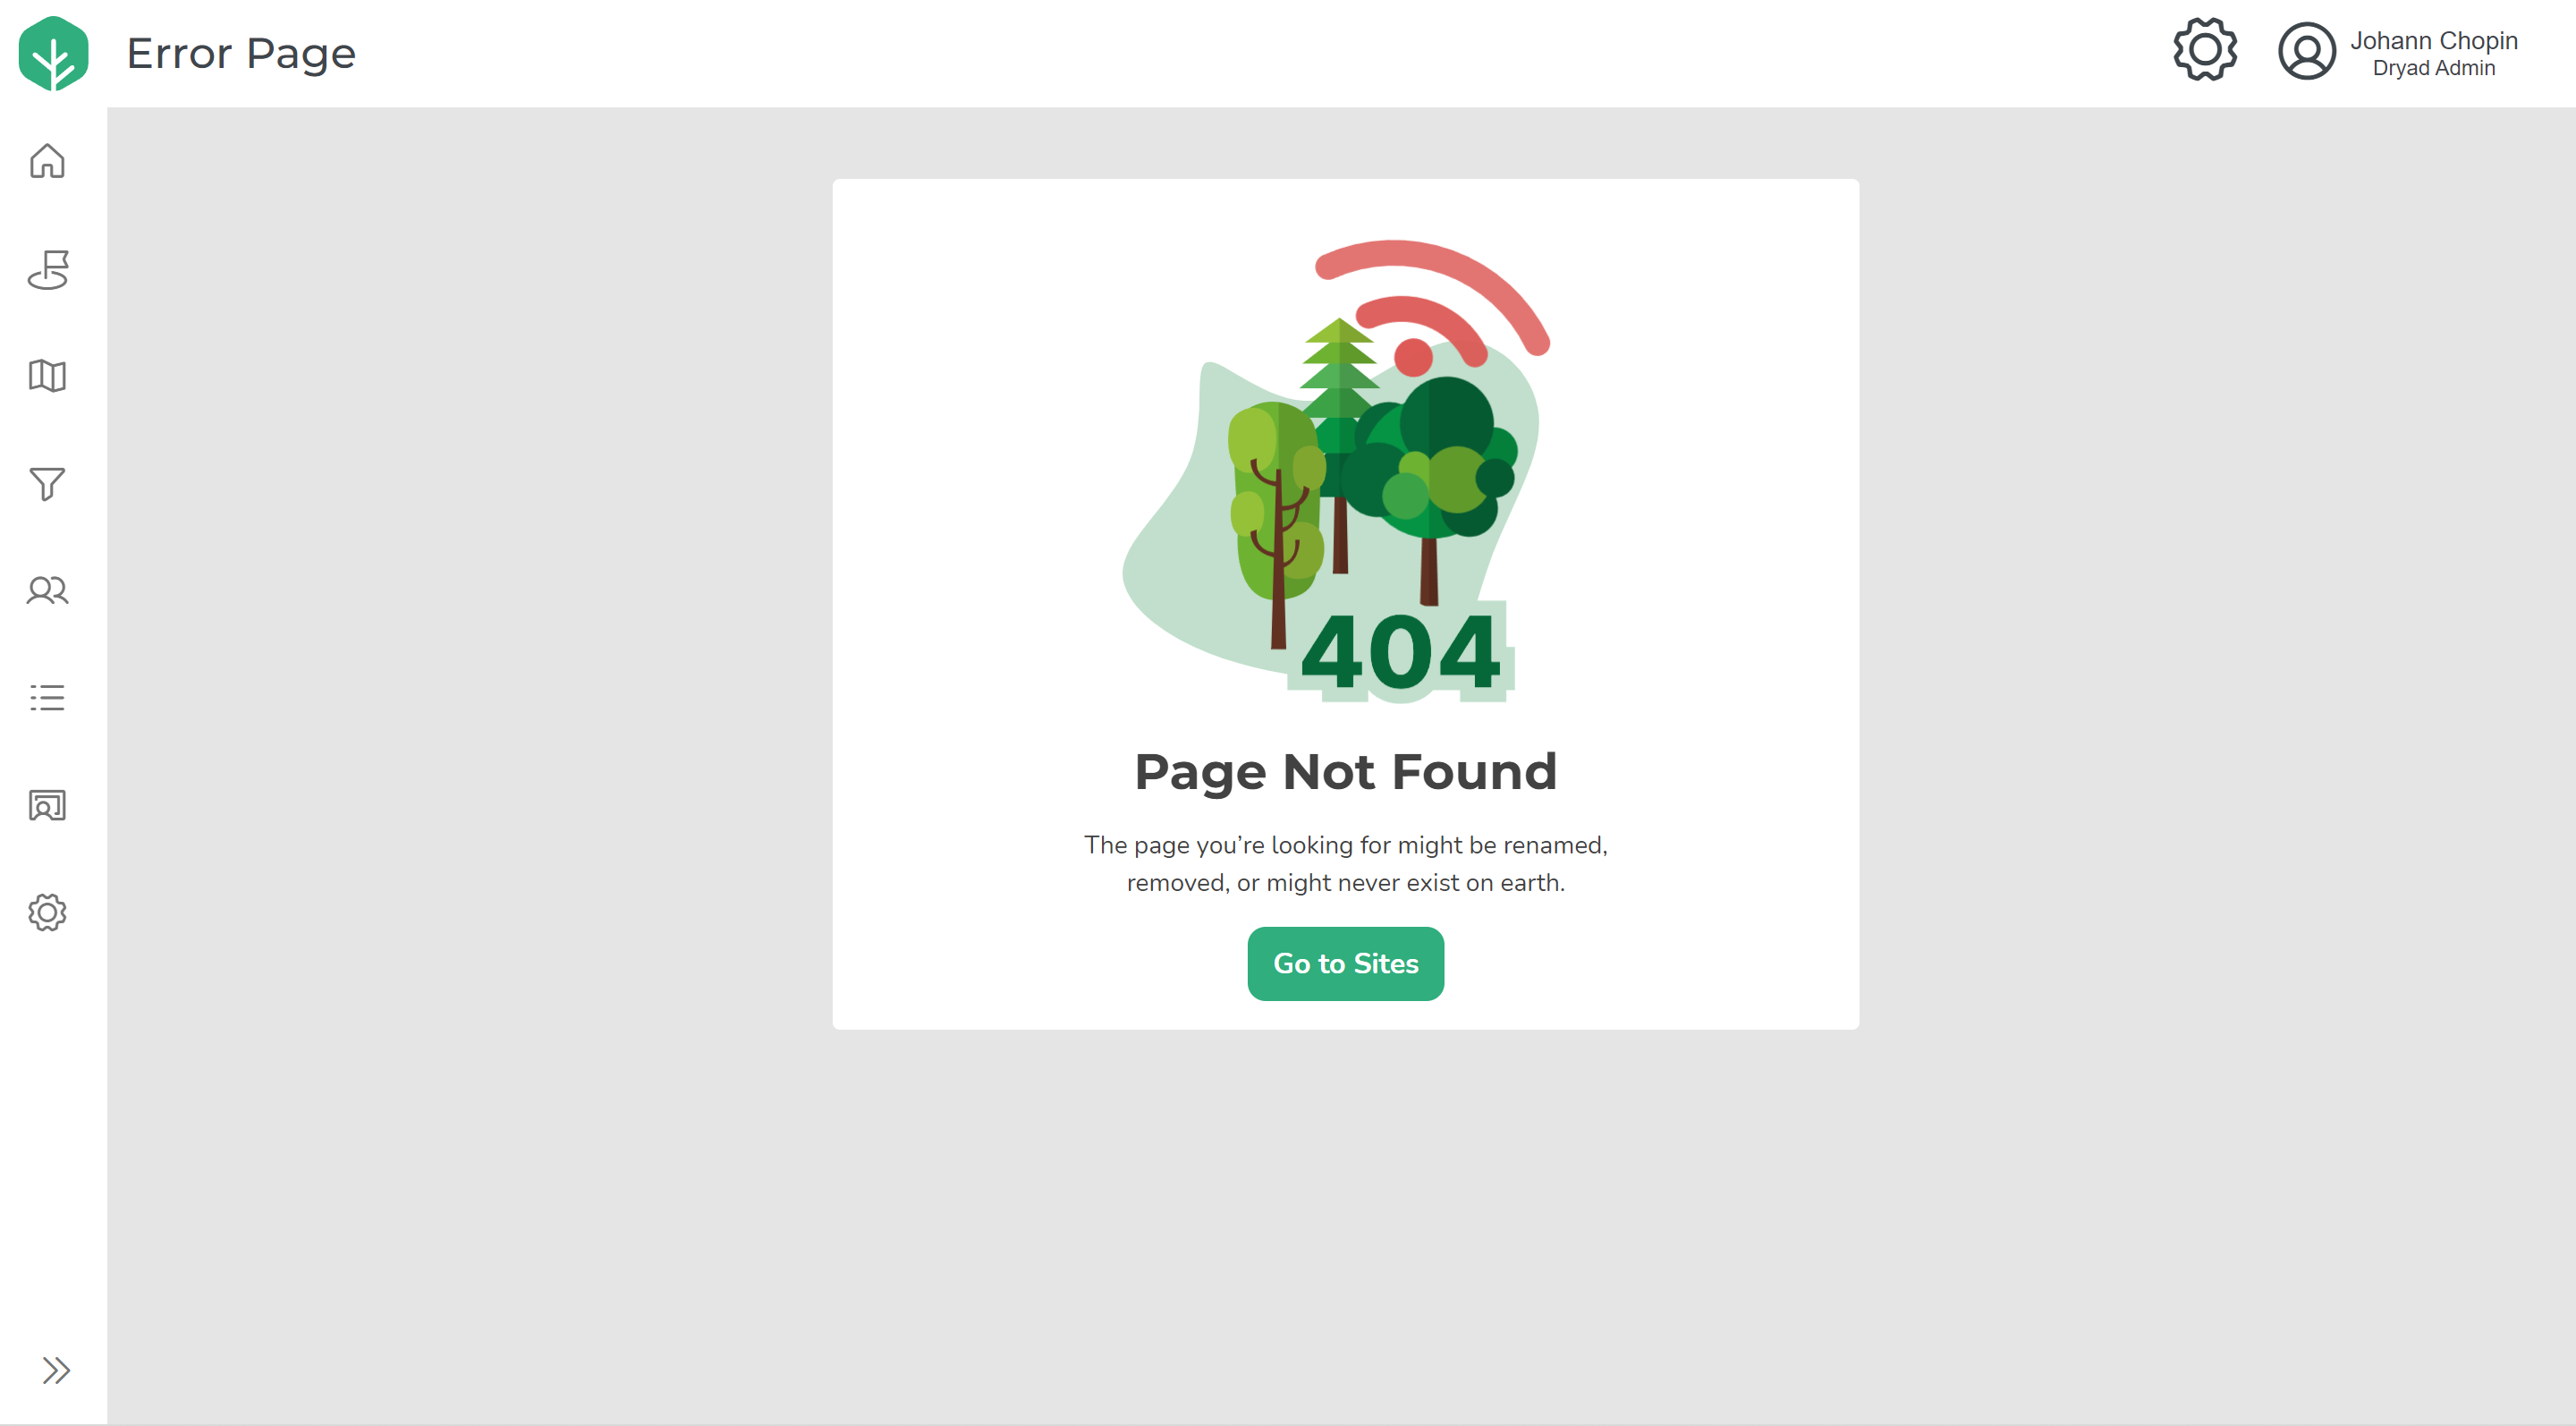
\includegraphics[width=13cm]{app_404_new}
  \caption{Prototyp der neuen 404-Seite}
  \label{fig:app_404_new}
\end{figure}

\begin{figure}[H]
  \centering
  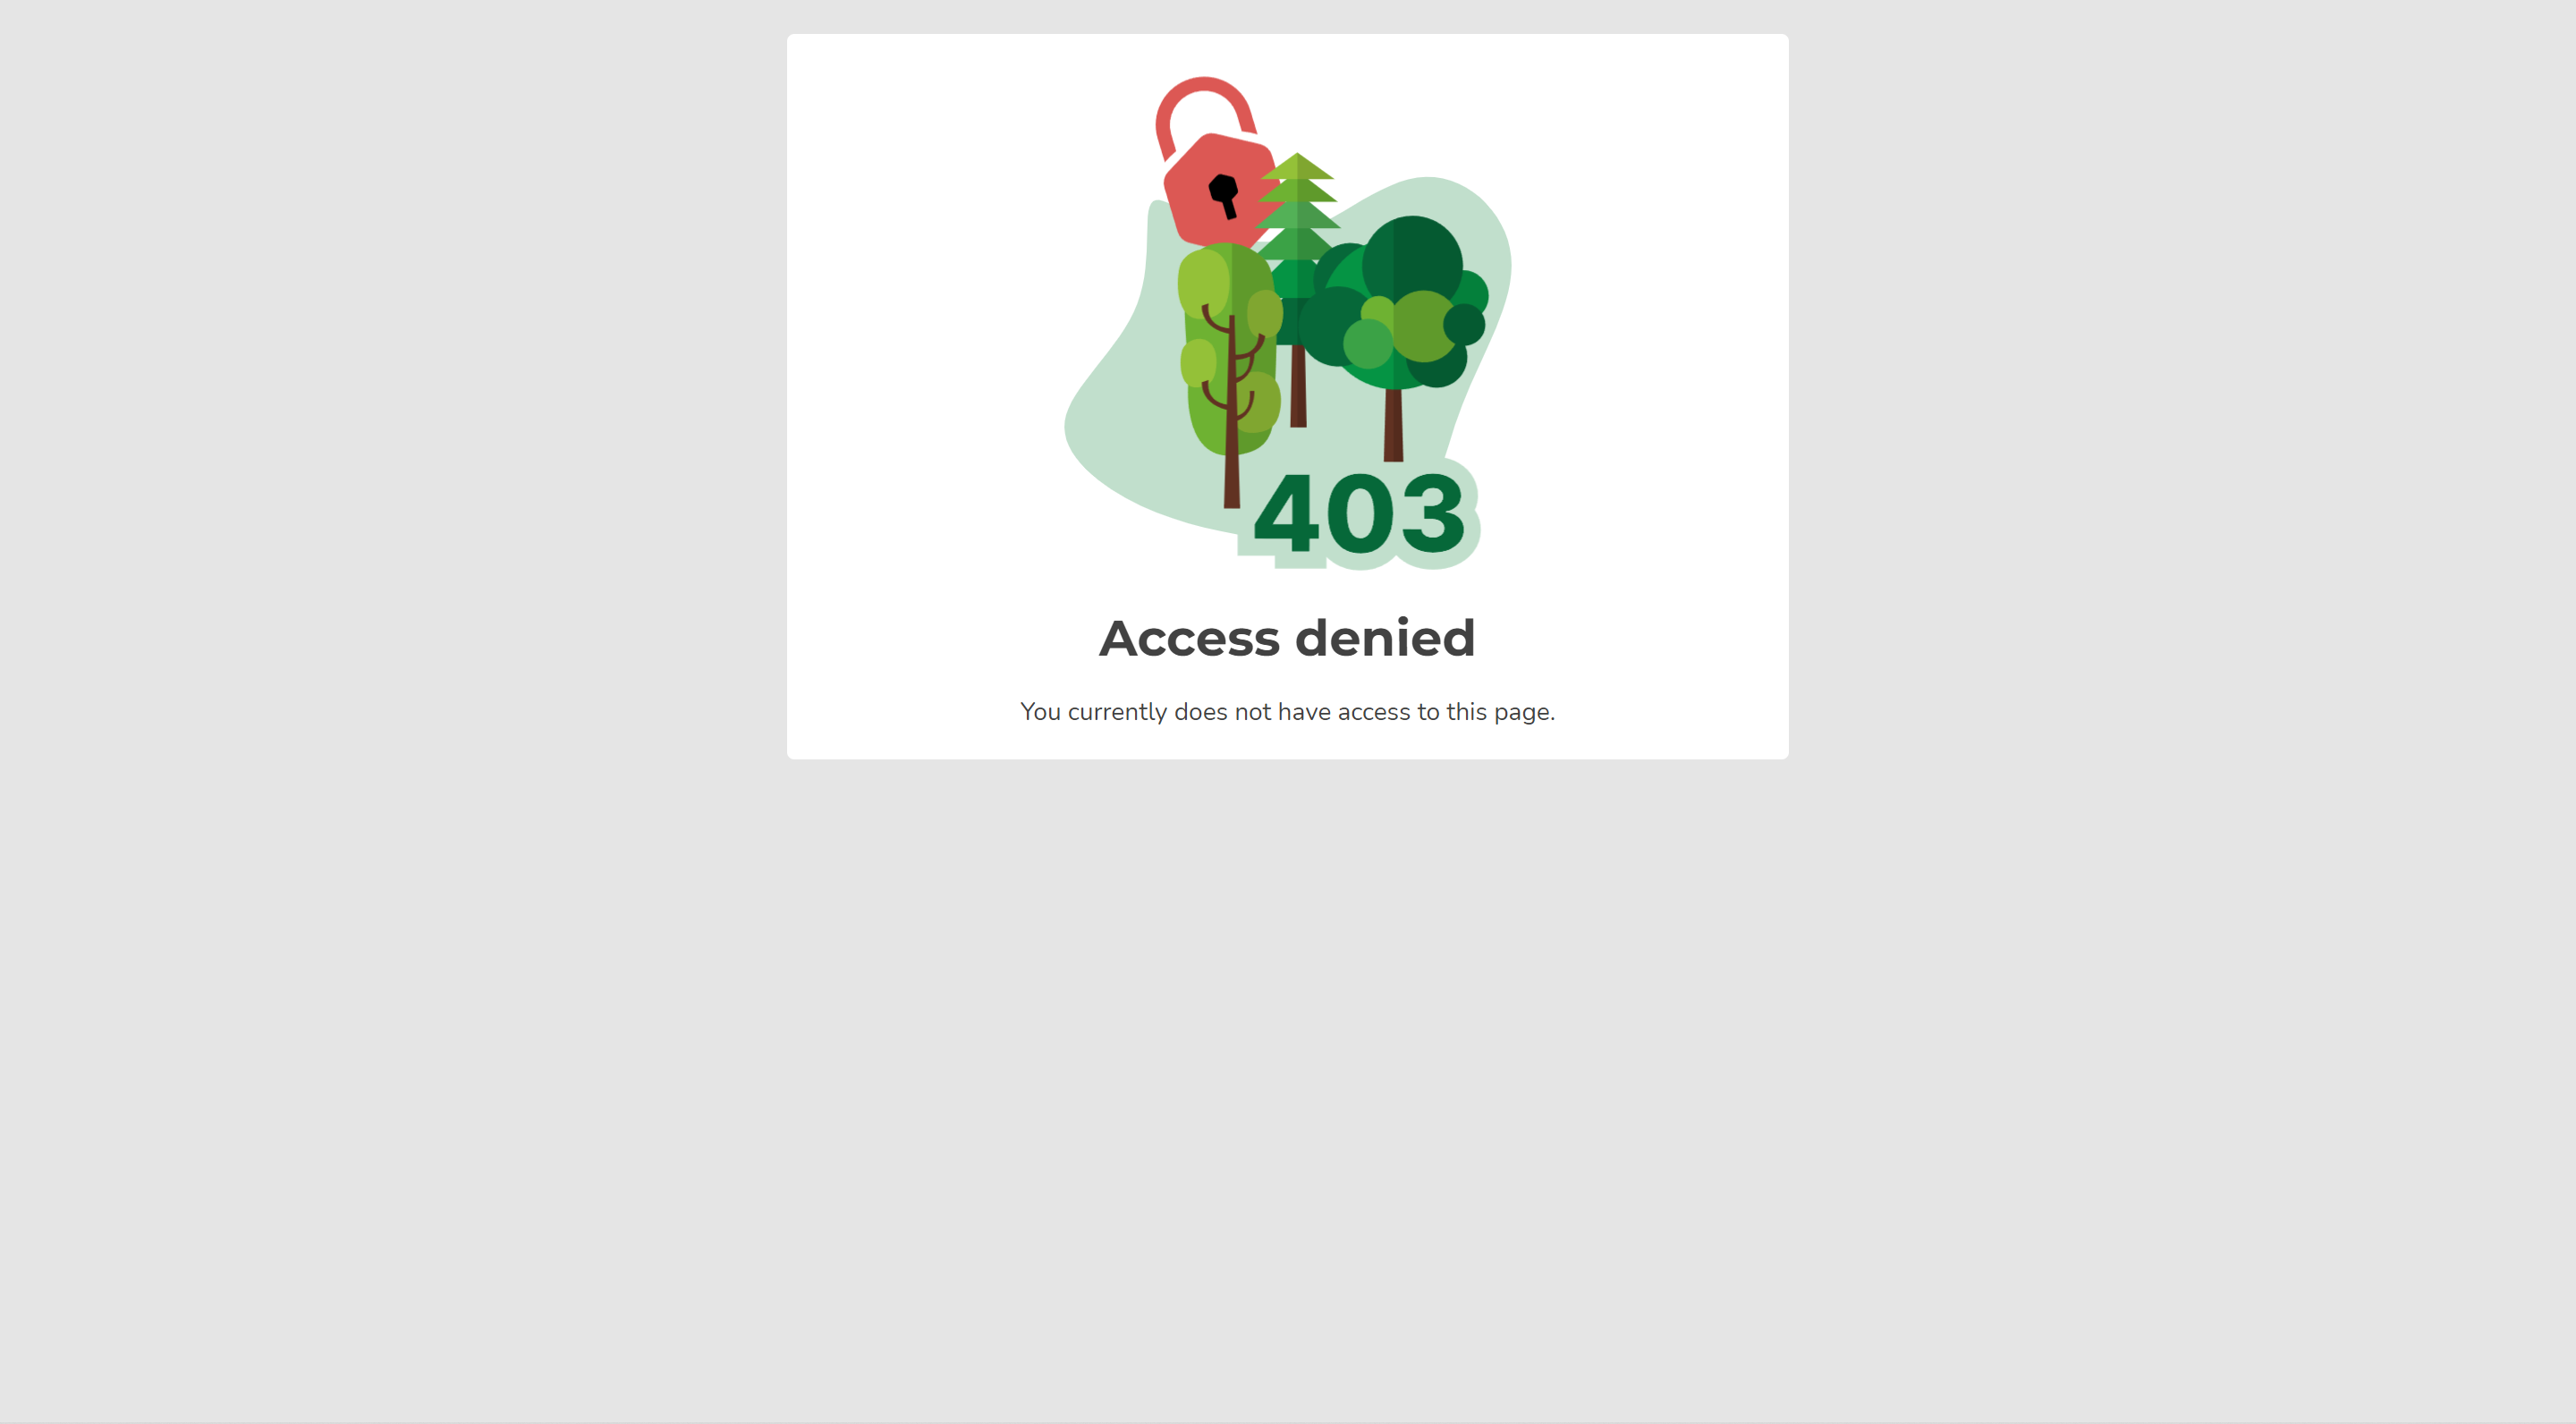
\includegraphics[width=13cm]{app_403}
  \caption{Prototyp der Seite, die einem Benutzer angezeigt wird, der versucht, ohne die erforderlichen Rechte auf eine Seite zuzugreifen.}
  \label{fig:app_403}
\end{figure}

\subsubsection{Darstellung der Stabilität}

Dieses UI-Design mit Illustrationen kann auch für andere Zwecke als die Anzeige von Fehlern verwendet werden.
Ein gutes Beispiel und die Alert-Seite, die von slug \lstinline{/alert-centre} aus verfügbar ist.
Wenn keine Warnmeldungen erkannt werden, ist die Seite einfach nur leer.
Wenn Sie in diesem Fall eine animierte Abbildung eines friedlichen Waldes mit den verschiedenen Sensoren des Silvanet-Systems hinzufügen, wird der Benutzer, wenn er sie sieht, beruhigt und die verfügbaren Produkte werden noch einmal hervorgehoben.

\begin{figure}[H]
  \centering
  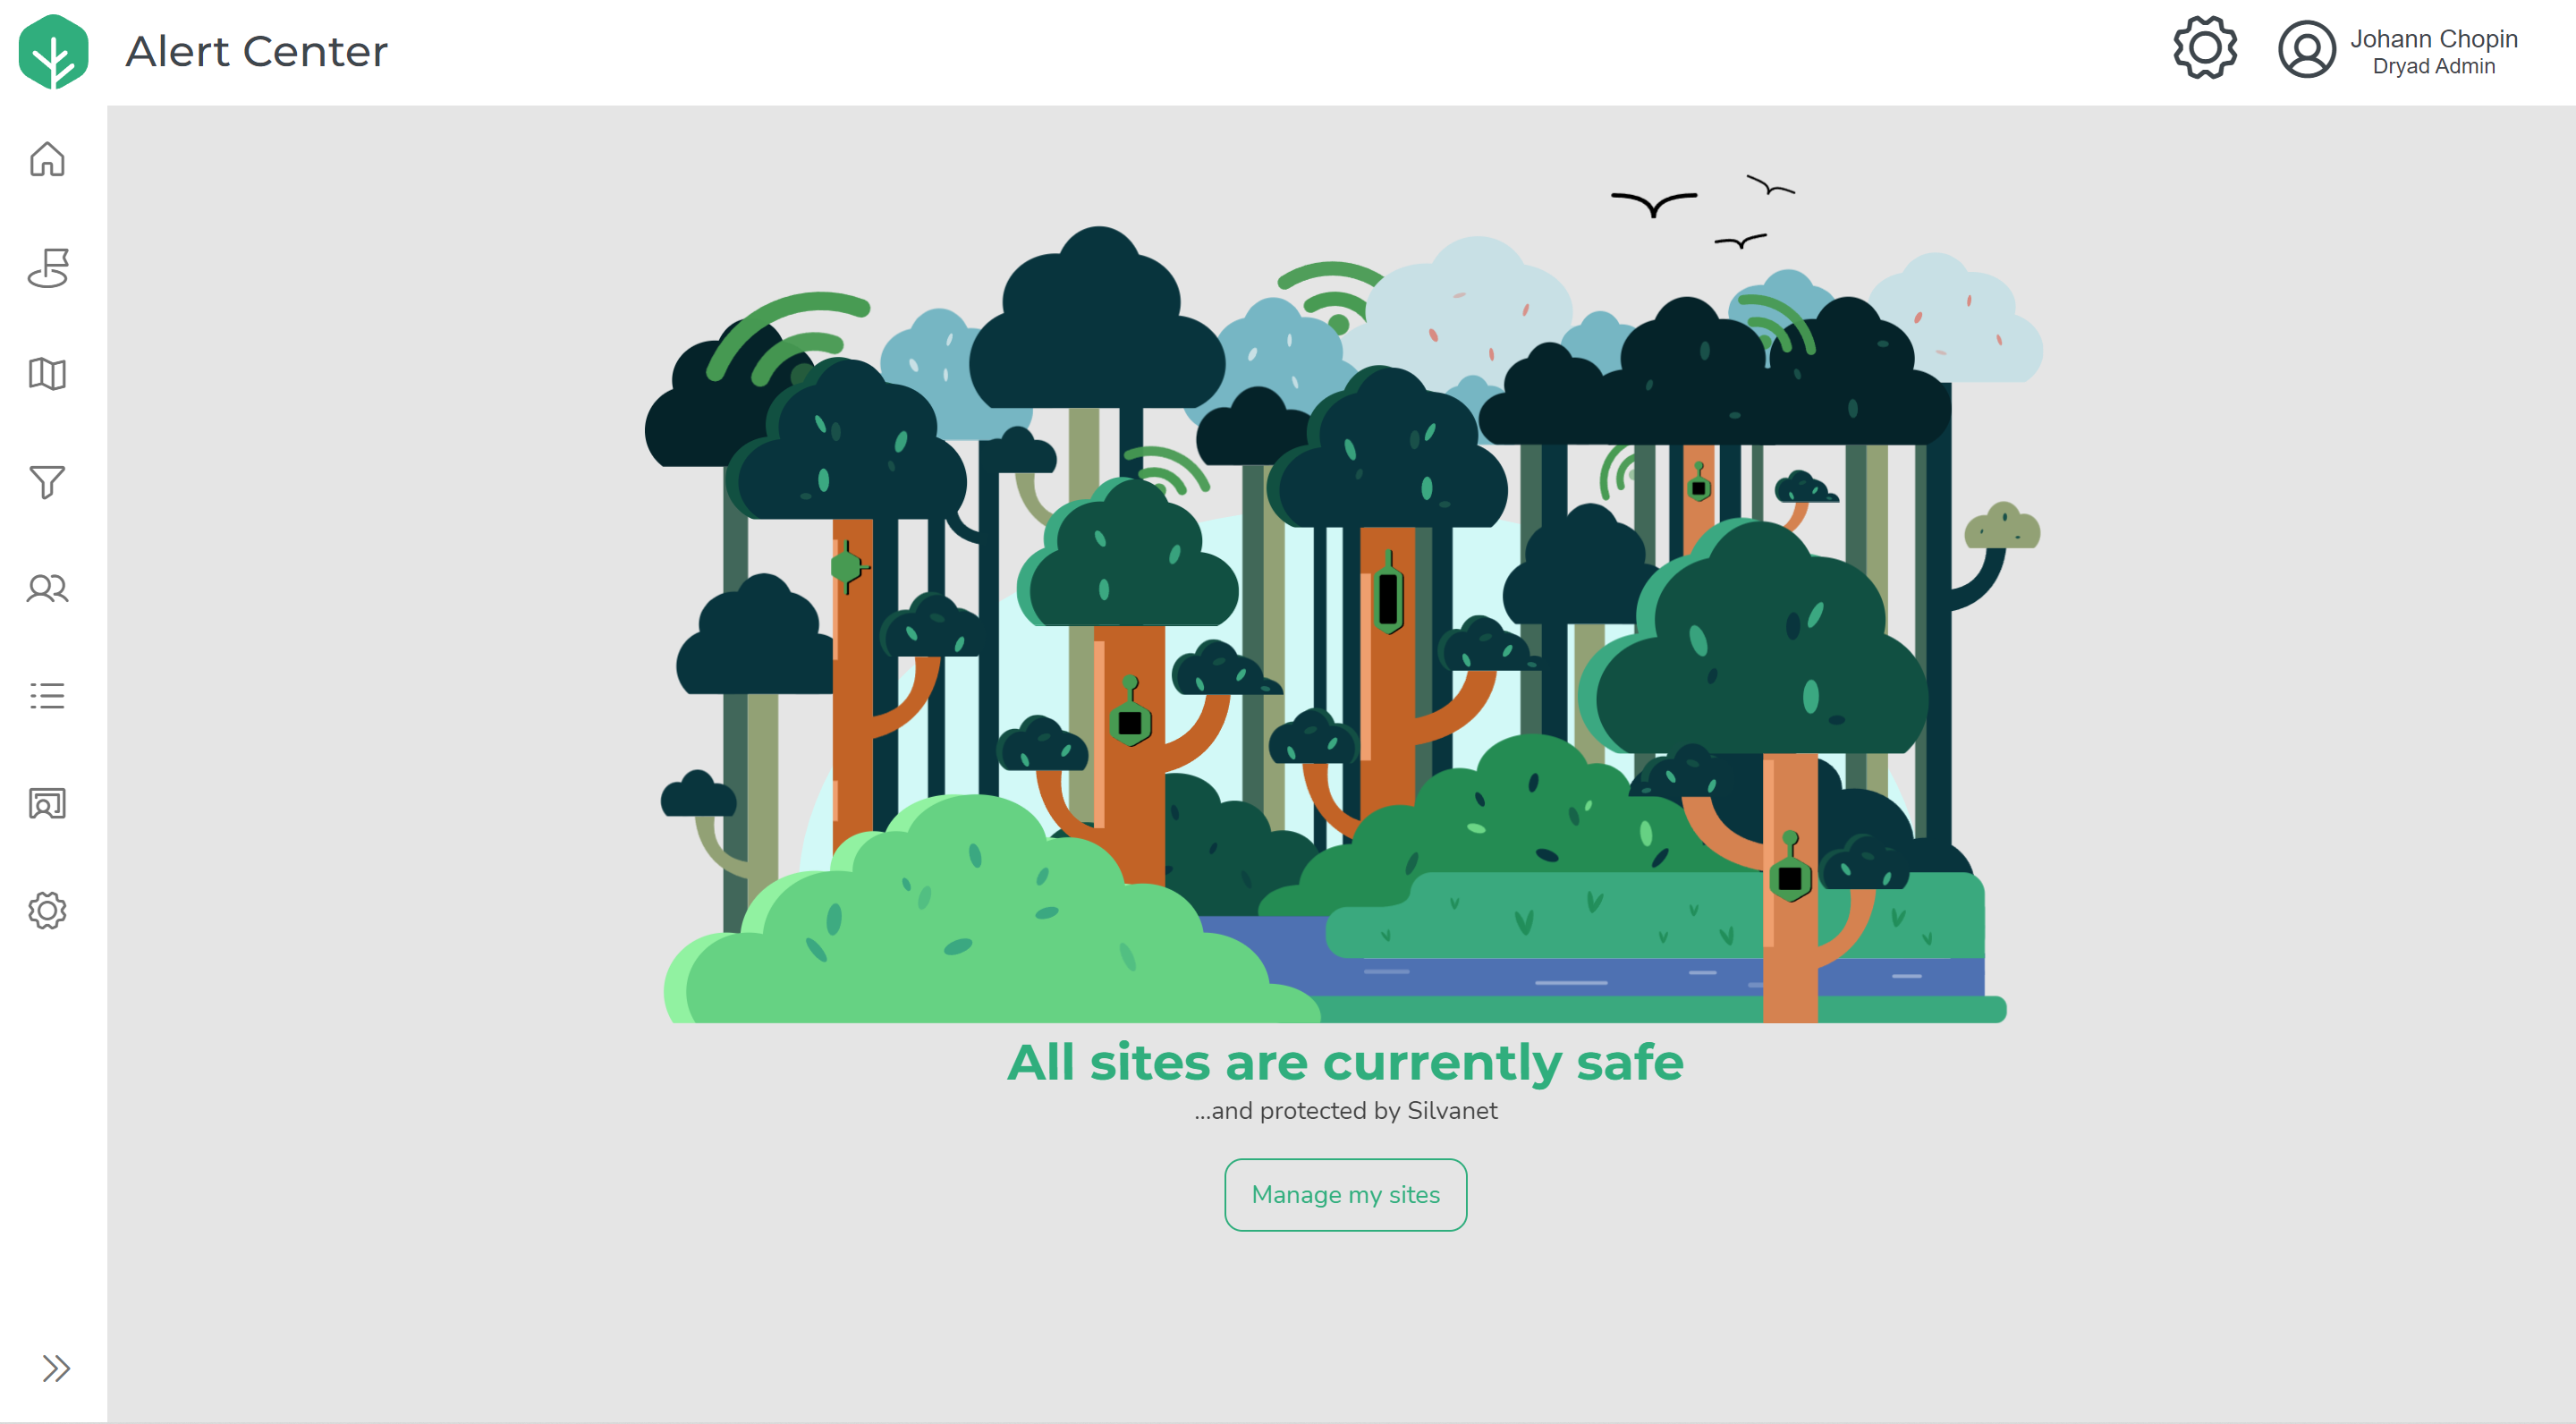
\includegraphics[width=\textwidth]{app_alert_center_safe}
  \caption{Seite des Alert-Centers, auf der angezeigt wird, dass derzeit keine Alerts detektiert werden}
  \label{fig:app_alert_center_safe}
\end{figure}

\subsubsection{Mechanismus zur Alarmierung bei Feuererkennung}

Wenn das Silvanet-System einen Waldbrandalarm erkennt, wird eine E-Mail an alle Personen gesendet, die als Verantwortliche für den betreffenden \textit{Site} aufgelistet sind.
Auf der Webschnittstelle kann man sich über ein Echtzeitsystem auch anzeigen lassen, wenn eine Alarmierung erkannt wurde.
Sie ist mit einem Websocket-Kanal verbunden, der es ermöglicht, in Echtzeit verschiedene Informationen zu empfangen und zu versenden, insbesondere Warnungen vor Waldbränden.
Wenn ein Alert auftritt, blinkt derzeit im Header der Seite ein Link, der zur Seite des Alert Centers weiterleitet (siehe \ref{fig:app_fire_alert_button_badge}).
Benutzertests haben gezeigt, dass die Anzeige der Anzahl der Alarme (entsprechend der Anzahl der Sensoren, die Rauch erkennen) für den Benutzer verwirrend war, da er nicht wusste, was er von dieser Zahl halten sollte.
Außerdem führt das rote Design des \ac{UI}-Elements und seine Blinkanimation dazu, dass der Nutzer sehr schnell und natürlich darauf klickt, ohne sich wirklich die Zeit zu nehmen, das Vorhandensein dieser Zahl zu identifizieren.
Da diese Nummer keinen Mehrwert bietet, überfrachtet sie die Benutzeroberfläche und kann daher entfernt werden. Außerdem sollte ein Flammen-Icon verwendet werden, um das Konzept des Feuers zu standardisieren.

\begin{figure}[H]
  \centering
  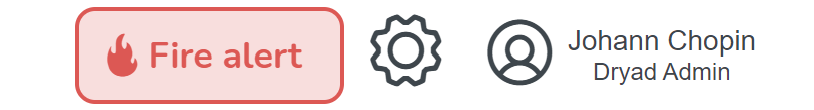
\includegraphics[width=6cm]{app_fire_alert_button_v2}
  \caption{Prototyp der vereinfachten Schaltfläche zur Meldung einer Warnung}
  \label{fig:app_fire_alert_button_v2}
\end{figure}

Benutzertests zeigen, dass dieses \ac{UI}-Element sehr effektiv ist, um einen Alarm zu melden, wenn sich der Benutzer auf der Oberfläche befindet.
Leider ist diese Funktion nur dann nützlich, wenn sich der Benutzer auf der Anwendungsseite seines Browsers befindet.
Wenn der Nutzer eine andere Registerkarte seines Browsers besucht, ist er nicht in der Lage, höchstens eine Warnung zu erkennen.
Es ist jedoch möglich, die Aufmerksamkeit des Nutzers auf einen bestimmten Tab zu lenken, auch wenn er inmitten vieler anderer Tabs untergeht.
Jede Webseite wird in einem Tab durch ihren Titel und ein kleines Icon, das sogenannte \textit{Favicon}, symbolisiert.
Sie können dieses Favicon genauso blinken lassen wie die Schaltfläche, die zum Warnzentrum weiterleitet, indem Sie das Favicon standardmäßig mit demselben roten Favicon alarmieren, das die Gefahr anzeigt.
Das Gefahren-Favicon wird auch ein wenig von dem Standard-Favicon abweichen, so dass auch Menschen mit Problemen bei der Farberkennung eine Bewegung sehen können.

\begin{figure}[H]
  \centering
  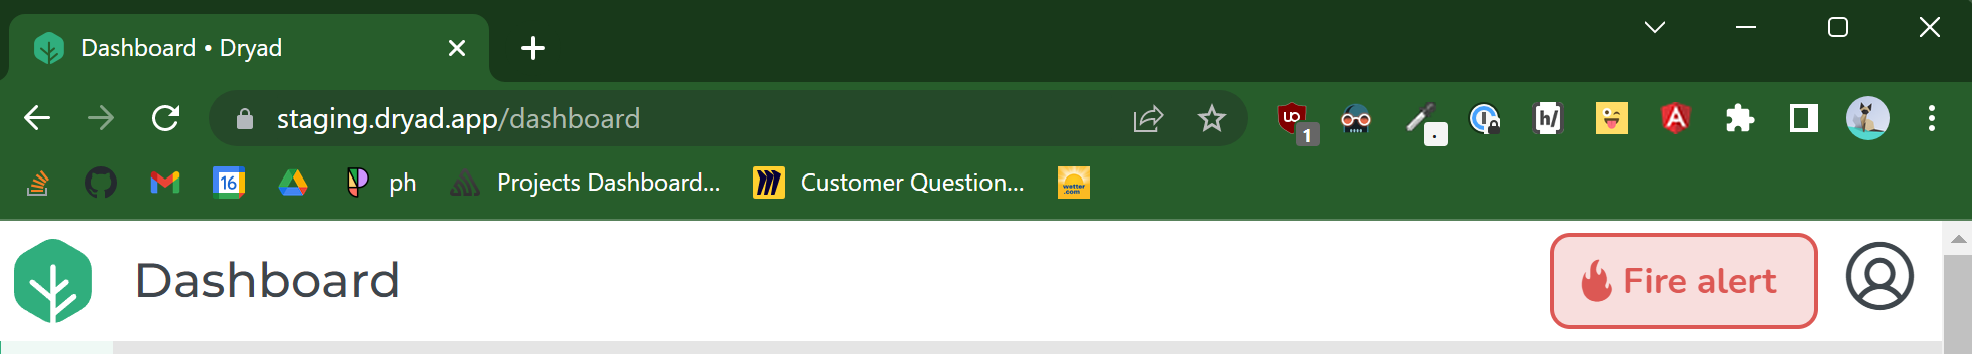
\includegraphics[width=\textwidth]{app_favicon_default}
  \caption{Standard-Favicon der Anwendung von Dryad (grünes Icon in der linken oberen Ecke)}
  \label{fig:app_favicon_default}
\end{figure}

\begin{figure}[H]
  \centering
  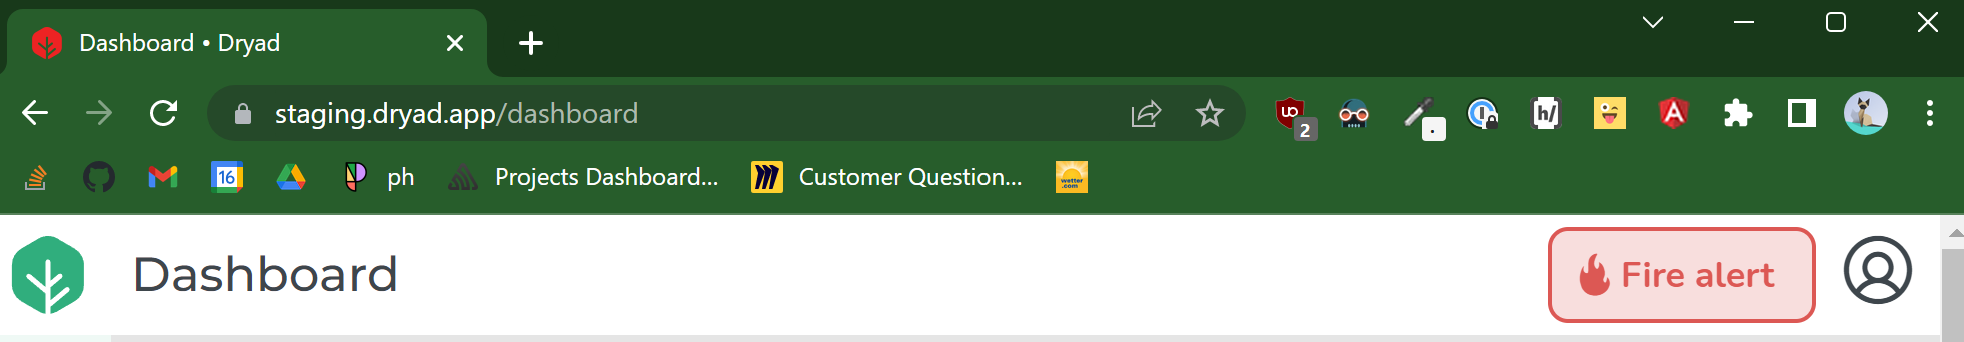
\includegraphics[width=\textwidth]{app_favicon_danger}
  \caption{Favicon der Dryad-App in einer roten Variante und leicht verschoben, um einen Tab mit einem Blinkeffekt hervorzuheben}
  \label{fig:app_favicon_danger}
\end{figure}

\subsection{Anwendungsanpassung und Lokalisierung}
Um dem Nutzer ein besseres Erlebnis zu bieten, ist es wichtig, dass sich die Benutzeroberfläche an den Nutzer anpasst und nicht umgekehrt.
Eine Anwendung sollte ein Werkzeug sein und nicht eine Einschränkung für den Nutzer.
Daher ist es sehr wichtig, dass sich die Schnittstelle automatisch anpasst oder angepasst werden kann, wo kulturelle Unterschiede auftreten.
Ein sehr auffälliges Beispiel ist die Anzeige von Entfernungsdaten, die nicht skaliert sind und ständig in metrischen Einheiten angezeigt werden.
So zeigt die Benutzeroberfläche immer wieder Daten wie die Fläche eines Geländes von 225300 Quadratmetern an, was dem Benutzer viel Mühe bereitet, sich diese Größe vorzustellen, während 22,53 Hektar viel leichter verdaulich sind.
Außerdem ist die Schnittstelle auch für den amerikanischen Markt bestimmt, der das Imperialsystem mit Einheiten wie Fuß, Meile oder Acre für Flächen verwendet.

In der gleichen Idee sollte es möglich sein, auszuwählen, wie das Datums- und Zeitformat angezeigt werden soll.
Die verschiedenen Optionen werden zwischen dem metrischen und dem imperialen System unterschieden.

\begin{table}[H]
  \centering
  \begin{tabular}{l c c}
    \toprule % Top horizontal line
                             & \multicolumn{2}{c}{\textbf{Messsystem}}                               \\
    \cmidrule(l){2-3}
    \textbf{Datentyp}        & Metrisches System                       & Imperialsystem              \\
    \midrule % In-table horizontal line
    Entfernungen und Flächen & m, km, und ha                           & ft, mile und acre           \\
    Datum                    & dd/mm/yyyy                              & yyyy-mm-dd                  \\
    Uhrzeit                  & 24-Stunden-Format (22:00)               & 12-Stunden-Format (10:00PM) \\
  \end{tabular}
  \caption{Einheitenformat, das auf dem metrischen oder imperialen System basiert}
\end{table}

Die Benutzeroberfläche sollte in der Lage sein, automatisch zu erkennen, welches Messsystem verwendet wird.
In einem zweiten Schritt sollte der Benutzer eine Seite mit Präferenzen erhalten, auf der er auswählen kann, welche Formate er für die verschiedenen Datentypen verwenden möchte.
Die automatische Erkennung erfolgt durch die Erkennung der Sprache des Browsers des Nutzers.
Wenn die Standardsprache amerikanisches Englisch ist, das in RFC5646 \cite{rfc5646} als \textit{en-US} bezeichnet wird, dann wird das imperiale System verwendet. Im umgekehrten Fall wird das metrische System verwendet.

Die Konvertierung zwischen den verschiedenen Größenordnungen von Entfernungen und Flächen sollte automatisch von der Schnittstelle vorgenommen werden, um dem Nutzer die relevanteste Darstellung zu bieten.
Dies ist recht einfach zu bewerkstelligen, da alle Daten in Metern für die Entfernungen und in Quadratmetern für die Einheiten angegeben sind.
Die verschiedenen Größenordnungen und ihre jeweiligen Einheiten in Abhängigkeit vom verwendeten System sind in den folgenden Tabellen aufgelistet.

\begin{table}[H]
  \centering
  \begin{tabular}{l c c}
    \toprule
                                  & \multicolumn{2}{c}{\textbf{verwendete Einheit}}                  \\
    \cmidrule(l){2-3}
    \textbf{Entfernung in Metern} & Metrisches System                               & Imperialsystem \\
    \midrule
    < 1000 Metern                 & Meter (m)                                       & Fuß (ft)       \\
    >= 1000 Metern                & Kilometer (km)                                  & Meilen (mile)  \\
  \end{tabular}
  \caption{Einheit, die je nach Größenordnung der Entfernung verwendet wird}
\end{table}

\begin{table}[H]
  \centering
  \begin{tabular}{l c c}
    \toprule
                                    & \multicolumn{2}{c}{\textbf{verwendete Einheit}}                      \\
    \cmidrule(l){2-3}
    \textbf{Fläche in Quadratmeter} & Metrisches System                               & Imperialsystem     \\
    \midrule
    < 10.000 Quadratmetern          & Quadratmeter (m²)                               & Quadratfuß (ft²)   \\
    >= 10.000 Quadratmetern         & Hektar (ha)                                     & Acre (acre)        \\
    >= 1.000.000 Quadratmetern      & Quadratkilometer (km²)                          & Quadratmeile (mi²) \\
  \end{tabular}
  \caption{Einheit, die je nach Größenordnung der Fläche verwendet wird}
\end{table}

\subsection{Design mit kognitivem Tunnelsystem}
